\begin{frame}{Network model overview}

  \vspace{0.3cm}
  \onslide<1-6>{\hfill\begin{overpic}[width=.3\textwidth]{%
    figures/fig2AD_network_1cell_targets_158-aniso.png}
        \put(27,100){\normalfont \normalsize anisotropic}
      \end{overpic}}\hfill%
  \onslide<3-6>{\begin{overpic}[width=.3\textwidth]{%
      figures/fig2AD_network_1cell_targets_158-rew.png}
        \put(33,100){\normalfont \normalsize rewired}
      \end{overpic}}\hfill%
  \onslide<4-6>{\begin{overpic}[width=.3\textwidth]{%
      figures/fig2AD_network_1cell_targets_14-dist.png}
        \put(5,100){\normalfont \normalsize distance-dependent}
      \end{overpic}\hfill}%

    \onslide<1-6>{\vspace{0.55cm}}
    \onslide<2-6>{\hfill\begin{overpic}[width=.3\textwidth]{%
    figures/tuned_aniso_netw_targets.png}
        \put(12,100){\normalfont \normalsize tuned anisotropic}
      \end{overpic}}\hfill%
  \onslide<5-6>{\begin{overpic}[width=.3\textwidth]{%
      figures/fig2AD_network_1cell_targets_144-rew_tuned.png}
        \put(33,100){\normalfont \normalsize rewired}
      \end{overpic}}\hfill%
  \onslide<6>{\begin{overpic}[width=.3\textwidth]{%
      figures/fig2AD_network_1cell_targets_30-tuned_dist.png}
        \put(5,100){\normalfont \normalsize distance-dependent}
      \end{overpic}\hfill}%


\end{frame}

\begin{frame}{Results -- Overrepresentation of reciprocal connections} 
  


   \only<1>{\vspace{0.3cm}%\begin{center}
  \only<1>{\begin{overpic}[width=.26\textwidth]{%
    figures/fig2AD_network_1cell_targets_158-aniso.png}
        \put(29,100){\normalfont \small anisotropic}
      \end{overpic}}%
  \only<1>{\begin{overpic}[width=.26\textwidth]{%
      figures/fig2AD_network_1cell_targets_158-rew.png}
        \put(35,100){\normalfont \small rewired}
      \end{overpic}}%
  \only<1>{\begin{overpic}[width=.26\textwidth]{%
      figures/fig2AD_network_1cell_targets_14-dist.png}
        \put(6,100){\normalfont \small distance-dependent}
      \end{overpic}}%
    % \end{center}
  }
    

  
  \only<1>{\vspace{0.2cm}
  \begin{figure}
    \centering
    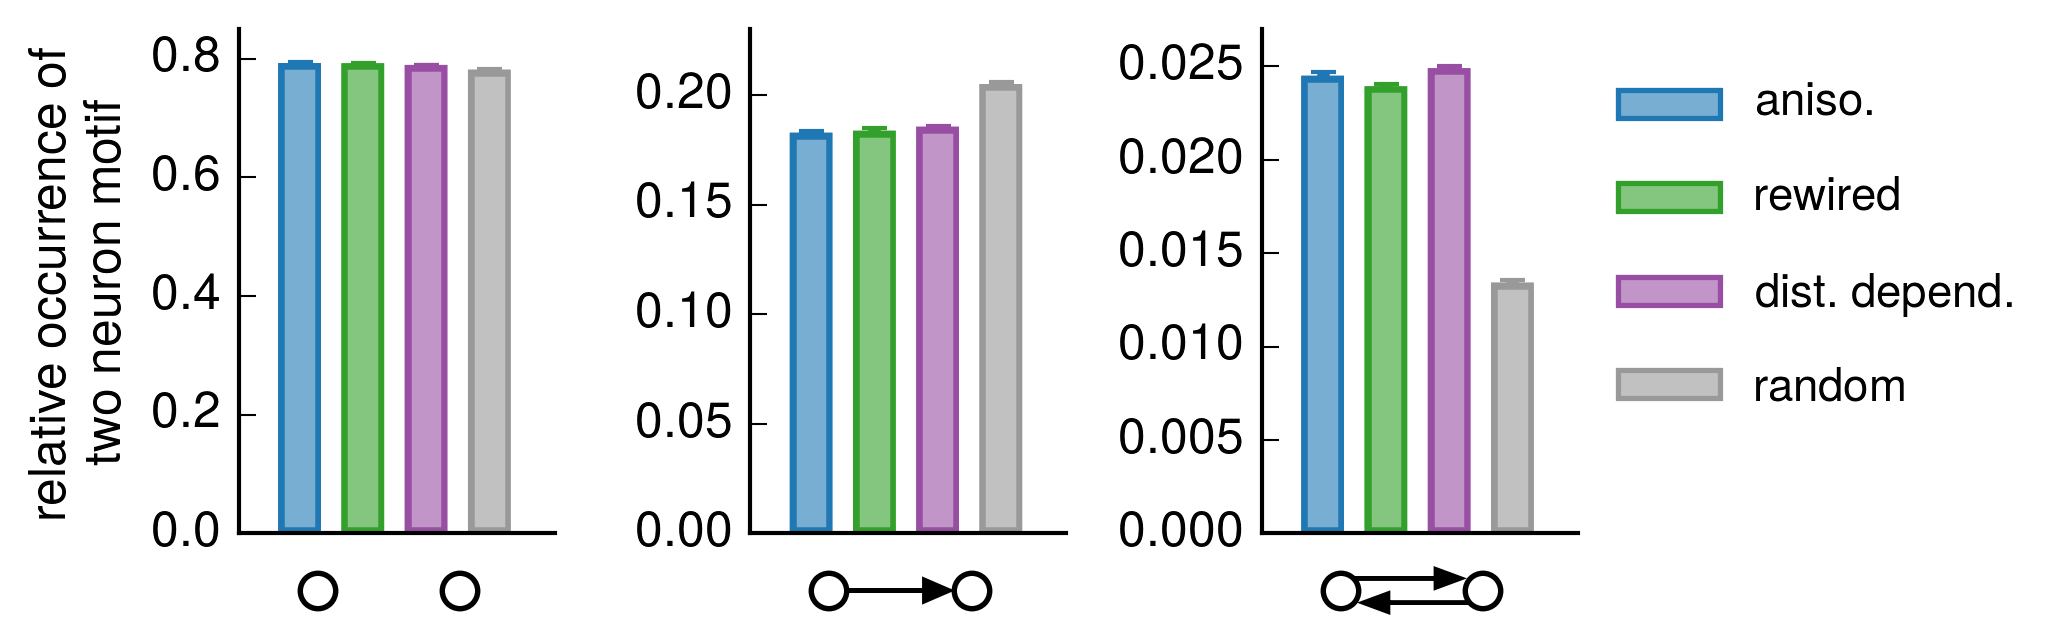
\includegraphics[width=0.95\textwidth]{%
      figures/fig3B_2n_rel_occurrence.png} %
  \end{figure}}


  \only<2-4>{
  \begin{figure}
    \centering
    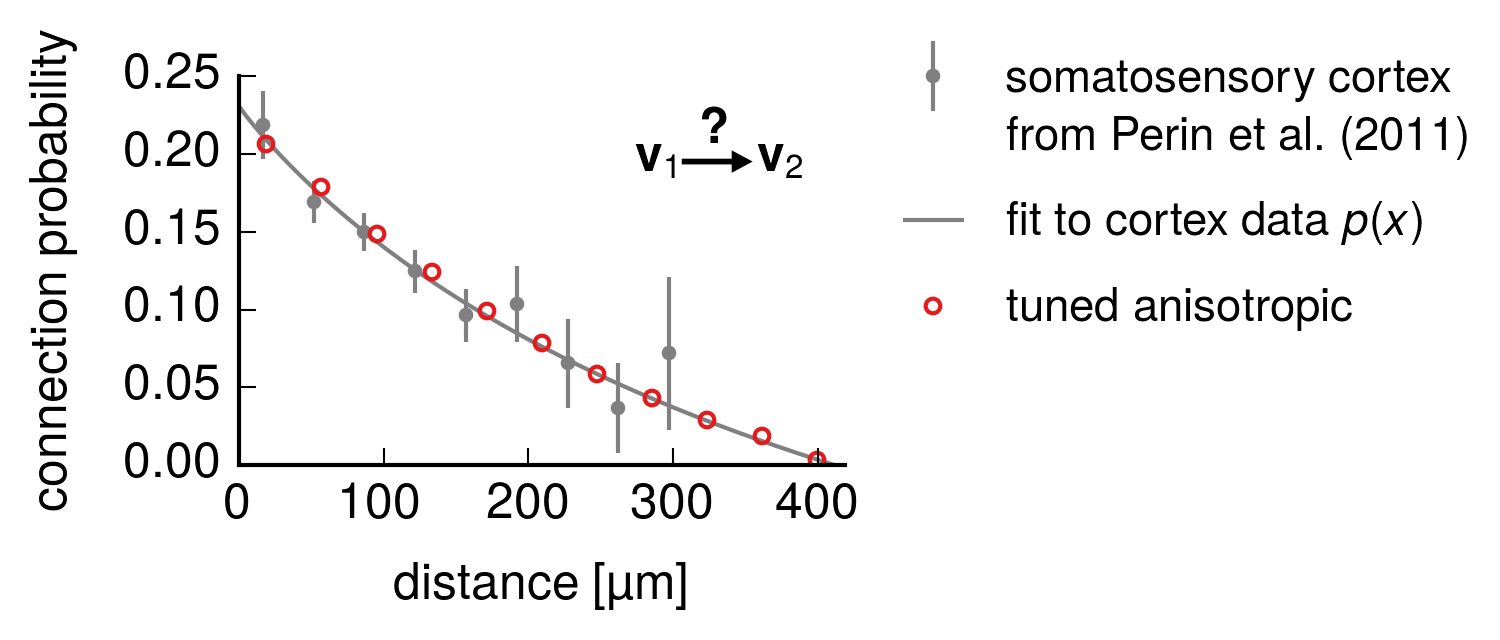
\includegraphics[width=0.88\textwidth]{%
      figures/fig3C_2n_dstprf.png}\\ %
    \includegraphics<2>[width=0.88\textwidth]{%
      figures/fig3D_recip_dist.png} %    
  \end{figure}}

  \only<3-4>{
    \begin{center}  
    % 
    \minipage[c][0.393\textheight][s]{0.8\textwidth}

    \vspace{0.6cm}
    
    {\large Other sources for the overrepresentation of bidirectional connections?}
    \vfill
    \onslide<4>
    \begin{arrowlist}
      \item {\large Hoffmann, FZ and Triesch, J (2017). Nonrandom
Network Connectivity Comes in Pairs. \textcolor{gray}{\textit{Network Neuroscience}}}
\end{arrowlist}

     \vspace{0.4cm}

     \endminipage
   \end{center}
  }

 
  % \source{Hoffmann \& Rotter, in prep.}
  
  
\end{frame}

